\documentclass[handout]{beamer}
\input{Lecture-Slides/preamble.txt}

% ------------------------------------------------------------
% Title Information
% ------------------------------------------------------------
\title{Introduction to Statistical Methods in Political Science}
\subtitle{Lecture 12: Small‑Sample Inference for Means: Student‑\textit{t} Toolbox}
\author{Ignacio Urbina \texorpdfstring{\\ \vspace{0.3em}}{ } 
        \scriptsize \textcolor{gray}{Ph.D.\ Candidate}}
\date{}

\begin{document}
\frame{\titlepage}

% ============================================================
% SECTION 0  WHY DO WE NEED NEW TOOLS?
% ============================================================
\section{From \textit{Z} to Student‑\textit{t}}

\transitionslide{Why Do We Need New Tools?}

% Motivation slide
\begin{frame}
\frametitle{Motivating example: Tiny Exit Poll}
\small
A survey team intercepts \textbf{12} early voters leaving a rural precinct.  They record time‑in‑booth (minutes) to study wait‑time equity. Longer time-in-booth may signal inefficiencies, understaffing, or barriers to quick voting (e.g., confusing ballots, slow machines).
\begin{itemize}
  \item Population SD \(\sigma\) is \emph{unknown}.  
  \item Sample histogram shows minor right‑skew and an outlier at 14 min.  
  \item Question: Can we still make a reasonably justified inference about the true mean wait time?
\end{itemize}
\pause
\textit{Z} procedures from last week assume:
\[
\text{Either } n\ge 30 \quad \textbf{or}\quad \sigma \text{ is known}.
\]
Neither is true here \(\Longrightarrow\) enter Student‑\textit{t}.
\end{frame}

%...............................................................................
% Conceptual slide
\begin{frame}
\frametitle{What actually changes when \(n\) is small?}
\begin{columns}[T]
\column{.43\textwidth}
\small 
\begin{itemize}
  \item We swap \(\sigma\) for the noisier estimate \(s\).  
  \item That extra “plug‑in” noise fattens the tails of our test statistic.  
  \item We can't rely on the ``plug-in principle'' (Law of Large Numbers doesn't hold).
  \item Student‑\textit{t} distribution captures this inflation with \textbf{degrees of freedom}:
        \[
        T=\frac{\bar X-\mu}{s/\sqrt n}\sim t_{df=n-1}
        \]
\end{itemize}

\column{.57\textwidth}
\centering
\vspace{2em}
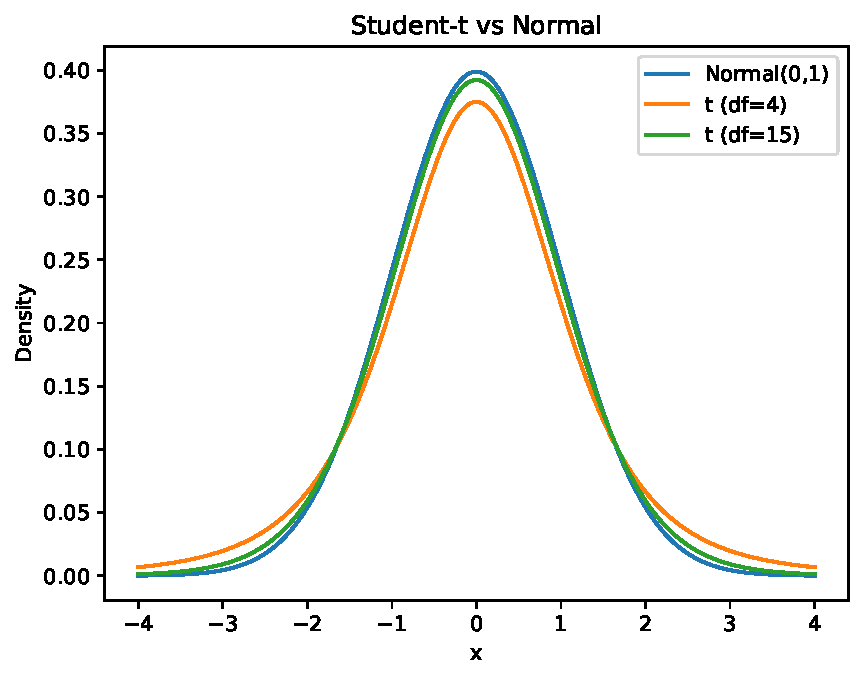
\includegraphics[width=\textwidth]{Figures/t_vs_norm.pdf}\\
\small (visual: \textit{t}\(_{\,4}\), \textit{t}\(_{\,15}\), and \(N(0,1)\))
\end{columns}
\end{frame}


%...............................................................................
\begin{frame}% Flowchart slide
\frametitle{Checklist before using a small-sample \textit{t} method}

\centering
\resizebox{\textwidth}{!}{%
\begin{tikzpicture}[
    >=Stealth,
    node distance = 1.4cm and 2.6cm,
    block/.style = {
        rectangle, draw, thick, rounded corners,
        align=center, minimum width=3.1cm, minimum height=1.1cm,
        inner sep=2pt
    },
    start/.style = {
        diamond, draw, thick, aspect=2, align=center,
        inner sep=2pt
    },
    edge_label/.style = {midway, sloped, font=\small, auto}
]

% ── Nodes ─────────────────────────────────────────────
\node (start) [start] {Start here};
\node (ind)   [block, below=of start] {Probabilistic Sampling \\ (e.g., SRS)};
\node (model) [block, right=of ind] {Model-based \\ adjustments \\ (weighting, MRP, …)};
\node (shape) [block, below=of ind] {Underlying shape \\ roughly normal?};

% Slight inward shift to tighten lower pair
\node (ok)  [block, below left=of shape,  xshift= .6cm] {Proceed \\ with \textit{t}};
\node (alt) [block, below right=of shape, xshift=-.6cm] {Consider \\ Other Methods \\ (bootstrap \\ or transformations)};

% ── Edges + labels ───────────────────────────────────
\draw[->, thick] (start) -- (ind);
\draw[->, thick] (ind)   -- node[edge_label] {yes} (shape);
\draw[->, thick] (ind)   -- node[edge_label] {no}  (model);

\draw[->, thick] (shape) -- node[edge_label] {yes} (ok);
\draw[->, thick] (shape) -- node[edge_label] {no}  (alt);

\end{tikzpicture}}% end resizebox
\end{frame}




% Diagnostic slide
\begin{frame}
\frametitle{Data‐shape diagnostics come first}
\vspace{-0.7em}
\begin{columns}
\column{.53\textwidth}
\begin{itemize}
  \item With \(n<30\) a single high outlier can wreck validity.  
  \item Always inspect a \textbf{histogram} and \textbf{QQ‑plot}.  
  \item Rule of thumb: mild skew is tolerable for \(n\ge 15\); heavy skew/outliers call for non‑parametrics or resampling.
\end{itemize}
\column{.45\textwidth}
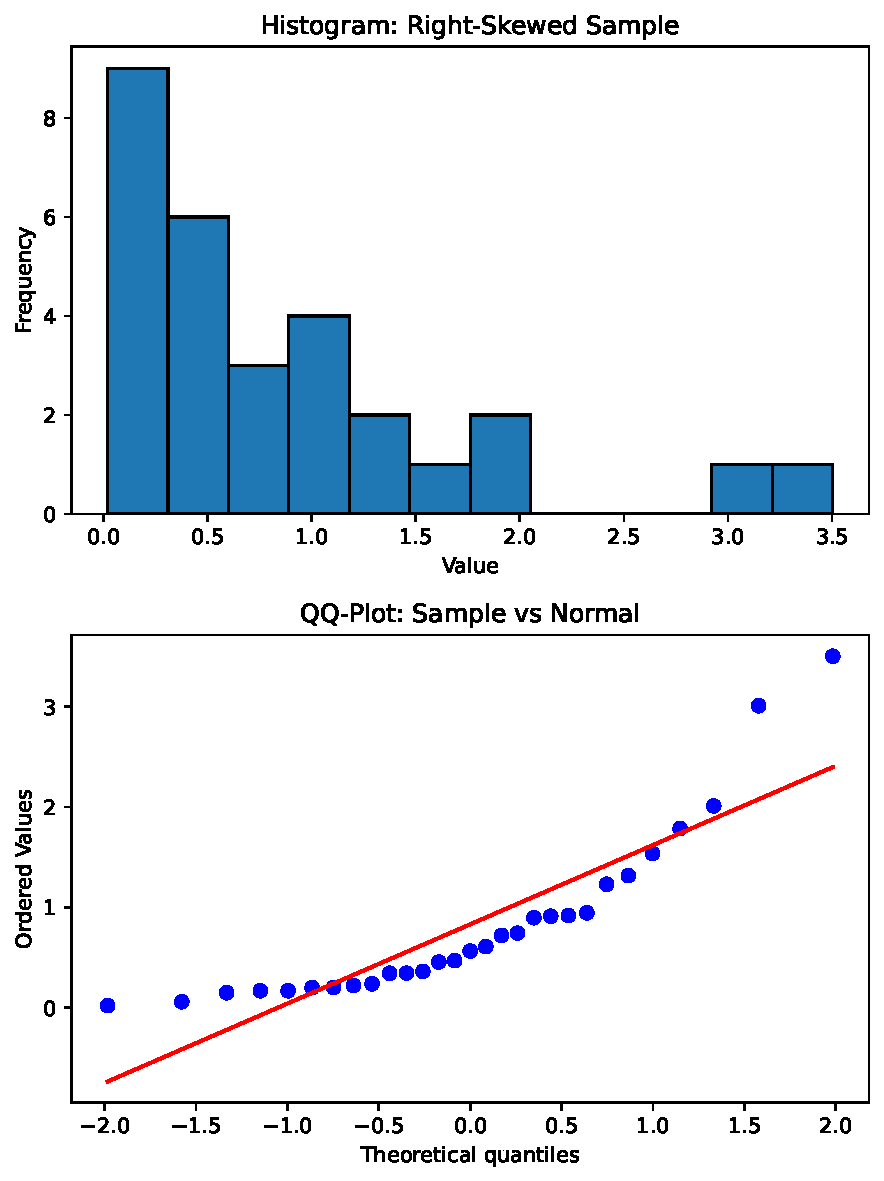
\includegraphics[width=\textwidth]{Figures/qq_example.pdf}
\end{columns}
\end{frame}

% .................................................................
% Intuition QQ plot
\begin{frame}
\frametitle{Intuition Behind a Q–Q Plot}
\begin{columns}[T,onlytextwidth]
  \column{0.48\textwidth}
  \textbf{What is a Q–Q plot?}
  \begin{itemize}
    \item Compares your data’s quantiles (y‑axis) to theoretical quantiles (x‑axis).
    \item If data follow the chosen distribution, points lie roughly on the 45° line.
    \item Deviations highlight skew, heavy tails, or outliers.
    \item Think of “lining up” your sample against the ideal.
  \end{itemize}

  \column{0.52\textwidth}
  \centering
  \textbf{QQ-Plot}
  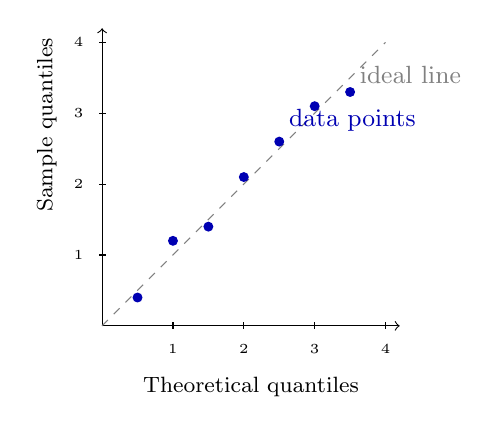
\begin{tikzpicture}[scale=0.9]
    % Axes with nicely spaced labels
    \draw[->] (0,0) -- (4.2,0) node[midway, below=15pt] {\footnotesize Theoretical quantiles};
    \draw[->] (0,0) -- (0,4.2) node[left=20pt, rotate=90] {\footnotesize Sample quantiles};

    % Reference line y=x
    \draw[dashed, gray] (0,0) -- (4,4);

    % Sample points (slightly off line)
    \foreach \x/\y in {0.5/0.4,1/1.2,1.5/1.4,2/2.1,2.5/2.6,3/3.1,3.5/3.3}
      \fill[blue!70!black] (\x,\y) circle(2pt);

    % Illustrative labels
    \node[font=\small, blue!70!black] at (2.5,2.6) [above right] {data points};
    \node[font=\small, gray] at (3.5,3.8) [below right] {ideal line};

    % Tick marks and tick labels
    \foreach \t in {1,2,3,4}{
      \draw (\t,0.05) -- (\t,-0.05) node[below,font=\tiny,yshift=-2pt] {\t};
      \draw (0.05,\t) -- (-0.05,\t) node[left,font=\tiny,xshift=-2pt] {\t};
    }
  \end{tikzpicture}
\end{columns}
\end{frame}


% .................................................................
\subsection{One‑Mean Confidence Interval}
% .................................................................
\transitionslide{One‑Sample CI for a Mean}

% ------------------------------------------------------------------
% Stand-alone slide: Sampling Distribution of the Sample Mean (Small $n$)
% ------------------------------------------------------------------
\begin{frame}
\frametitle{Sampling Distribution of Standardized $\bar{x}$ (Small Sample)}

\textbf{Goal:} Understand the behavior of $\bar{x}$ as an estimator of $\mu$ when sample size is small ($n < 30$).

\vspace{0.5em}
\textbf{Common assumptions}:
\begin{itemize}
  \item Data are collected via SRS.
  \item The population distribution is approximately Normal (key for small $n$ inference).
  \item Population SD ($\sigma$) is unknown.
\end{itemize}

\vspace{0.5em}
\textbf{Result:}
\[
\frac{\bar{x}-\mu}{s/\sqrt{n}}
 \sim t_{\,df=n-1} 
\]
\vspace{-0.5em}
\begin{itemize}
  \item Use $s$ to estimate $\sigma$ → introduces extra variability.
  \item The $t$ distribution accounts for this with heavier tails than Normal.
\end{itemize}

\end{frame}


\begin{frame}
\frametitle{Confidence Interval for $\mu$ in Small Samples -- The recipe}
\[
\boxed{\;
\bar{x} \ \pm\ t^{\ast}_{\,df=n-1,\,1-\alpha/2} \times
        \tfrac{s}{\sqrt n}
\;}
\]
\begin{itemize}
  \item \textbf{Degrees of freedom} \(df=n-1\).  
  \item \textbf{Critical value} \(t^{\ast}\) comes from a table or software.  It depends on both $df$ and $\alpha$.
  \item \textbf{Interpretation} follows the familiar “We are 95\% confident …”.
\end{itemize}
\end{frame}

% Interactive slide
\begin{frame}
\frametitle{Question – How does \(t^{\ast}\) compare with \(z^{\ast}\)?}
Suppose \(\alpha=0.05\).
\begin{enumerate}[A.]
  \item \(t^{\ast}_{\,19}\) is \textbf{smaller} than \(z^{\ast}=1.96\)  
  \item \(t^{\ast}_{\,19}\) is \textbf{equal to} \(z^{\ast}\)  
  \item \(t^{\ast}_{\,19}\) is \textbf{larger} than \(z^{\ast}\)  
  \item It cannot be determined because \(t^{\ast}\) depends on the sample’s standard deviation, whereas \(z^{\ast}\) does not  
\end{enumerate}
\pause
\textcolor{gray}{(Answer: C; heavier tails)}  
\end{frame}

% .................................................................
% Worked example
\begin{frame}
\frametitle{Worked example: Local campaign donors}
\vspace{-0.5em}
\begin{columns}[T]
\footnotesize
\column{.40\textwidth}
\textbf{Goal}: assess mean contributions, based on our sample of 18 local donors, by constructing a 90\% confidence interval for the mean donation.
\begin{itemize}
  \item \(n=18\), \(\bar x=\$42.8\), \(s=\$9.2\).  
  \item 90\% confidence wanted (\(\alpha=0.10\)).  
\end{itemize}
\pause
\textbf{Solution:}
\begin{align*}
t^{\ast}_{\,n-1,\,1-\frac{\alpha}{2}} &= t^{\ast}_{\,17,\,0.95}  = 1.740 \\
SE &= \frac{9.2}{\sqrt{18}} = 2.17 \\
ME &= 1.740\times2.17 = 3.77
\end{align*}
CI:\; \(\$42.8 \pm 3.8 = (\$39.0,\ \$46.6)\).
\column{.55\textwidth}
\vspace{3em}
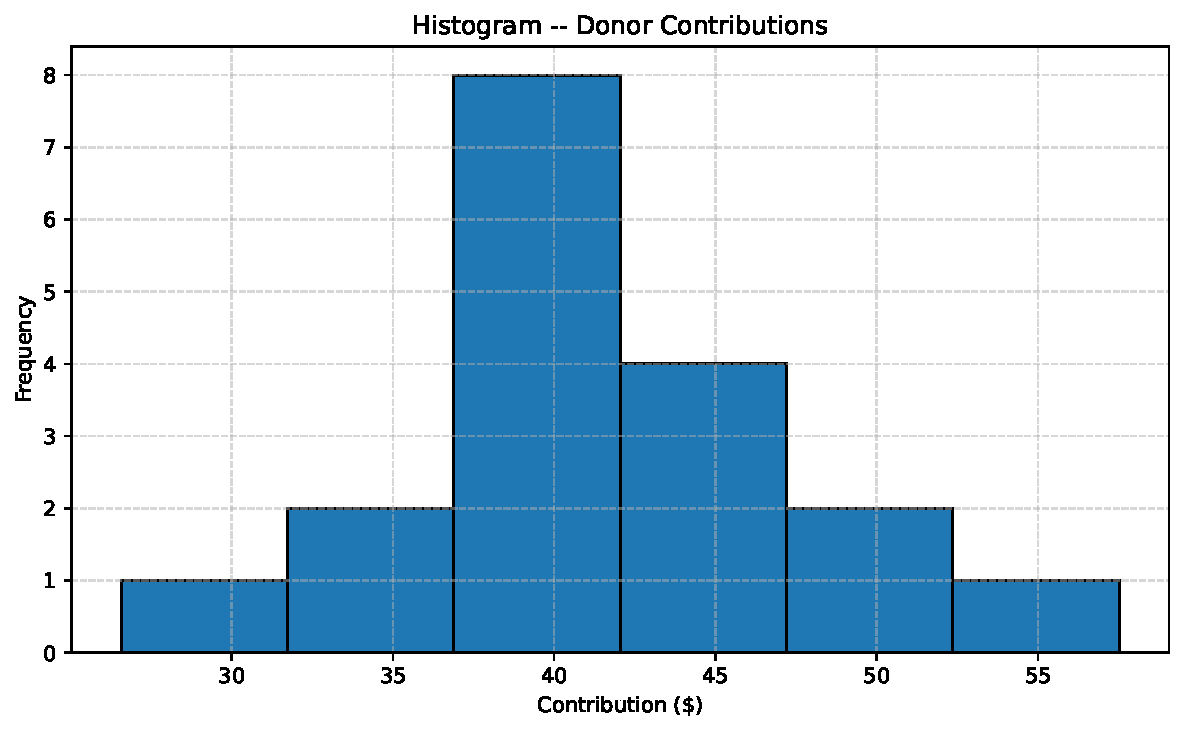
\includegraphics[width=\textwidth]{Figures/donor_hist.pdf}
\end{columns}
\end{frame}


% ============================================================
% SECTION — Hypothesis Testing for Means
% ============================================================
\section{Hypothesis Testing for Means}

% Transition slide

\transitionslide{Hypothesis Testing for Means}


% ------------------------------------------------------------
% 1.  Framework refresher
% ------------------------------------------------------------
\begin{frame}
\frametitle{Five–Step Road Map}
\begin{enumerate}
  \item \textbf{State \(H_0\) and \(H_a\)}   (parameter language, direction -- one or two tailed)\\[0.2em]
  \item \textbf{Choose \(\alpha\)}           (tolerable Type I risk)\\[0.2em]
  \item \textbf{Compute test statistic}     \(T=\dfrac{\text{estimate}-\text{null}}{SE}\)\\[0.3em]
        \(T\sim t_{df}\) if checklist passes.\\[0.2em]
  \item \textbf{Decision rule}  — compare either \(|T|\) to a critical value \(t^{\ast}_{df}\) \emph{or} use a \(p\)-value.\\[0.2em]
  \item \textbf{Conclusion in context}.     (plain‑English, mention evidence strength)
\end{enumerate}
\end{frame}

% ------------------------------------------------------------
% 2.  One‑sample t test
% ------------------------------------------------------------
\subsection{One‑Sample Test}

% Problem slide
% Problem slide
\begin{frame}
\frametitle{Worked Example — Average Time in Booth}
\small
\textit{Rural exit‑poll revisit.}  

\vspace{0.5em}
In response to concerns about unequal voting experiences, electoral officials assert that average time spent in the voting booth should not exceed \textbf{6 minutes}. They claim that rural polling stations are operating efficiently and equitably.

\vspace{0.5em}
Activists, skeptical of this claim, conduct an informal audit by collecting a small \textbf{simple random sample} of \(n=12\) early voters at a rural precinct. Each voter is asked how long they spent in the booth, from entry to casting their ballot.

\vspace{0.5em}
\begin{itemize}
  \item Sample mean: \(\bar x = 7.8\) minutes  
  \item Sample standard deviation: \(s = 3.1\) minutes  
  \item Officials’ claim: \(\mu = 6\) minutes (true average time)
\end{itemize}

\vspace{0.5em}
\textbf{Goal}: Test whether the true mean booth time \(\mu\) differs from 6 minutes. Use a two-sided \(t\) test at significance level \(\alpha = 0.05\).
\end{frame}

%.....................................................................................
% Calculation slide
\begin{frame}
\frametitle{Worked Example – 5‑Step Procedure}
\footnotesize

\textbf{Step 1: State hypotheses}\\[0.2em]
\quad \(H_0: \mu = 6\) minutes \hfill (official claim)\\
\quad \(H_a: \mu \neq 6\) minutes \hfill (activists suspect difference)

\vspace{1em}
\textbf{Step 2: Set significance level}\\[0.2em]
\quad \(\alpha = 0.05\) (two-tailed test). Hence, Critical value: \(t^{\ast}_{0.975,\,11} = 2.201\).

\vspace{1em}
\textbf{Step 3: Compute test statistic}\\[0.2em]
\quad Sample mean: \(\bar{x} = 7.8\), \quad sample SD: \(s = 3.1\), \quad \(n = 12\)\\
\quad Standard error: \(SE = \frac{3.1}{\sqrt{12}} = 0.90\)\\
\quad Test statistic: \(T = \frac{7.8 - 6}{0.90} = 2.00\)

\vspace{1em}
\textbf{Step 4: Make decision}\\[0.2em]
\quad Degrees of freedom: \(df = 12-1= 11\). Critical value: \(t^{\ast}_{0.975,\,11} = 2.201\)\\
\quad Since \(|T| = 2.00 < 2.201\), we \textbf{fail to reject} \(H_0\)

\vspace{1em}
\textbf{Step 5: Conclusion in context}\\[0.2em]
\quad Evidence is insufficient (at the 5\% level) to conclude that the true average booth time differs from the official 6-minute claim.

\end{frame}



% ============================================================
% SECTION —  PAIRED SAMPLES
% ============================================================

% .................................................................
\section{Paired‐Sample Confidence Interval}
% .................................................................

\transitionslide{Inference for Means in Paired‐Samples}


\begin{frame}
\frametitle{Why Use Paired Measurements?}
\small
\vspace{-0.3em}
\textbf{Context:} In many research settings, it's hard to detect a treatment effect when individual baseline differences are large.  
\\[0.6em]
\textbf{Solution:} \textbf{Pairing} allows each subject (or unit) to serve as their own control.

\vspace{1em}
\textbf{Common examples of pairing:}
\begin{itemize}
  \item \textbf{Before vs. after} a treatment or policy change (e.g., turnout before/after voter ID law)
  \item \textbf{Twin studies} in medical or behavioral research (genetically matched units)
  \item \textbf{Matched groups or regions} — e.g., similar counties, classrooms, or districts
\end{itemize}
\end{frame}

\begin{frame}
\frametitle{Why Use Paired Measurements?}
\textbf{Why it works:}
\begin{itemize}
  \item Controls for \textit{individual-level variability} (age, baseline attitudes, income, etc.)
  \item Focuses analysis on the \textbf{within-pair difference} \(d_i\)
  \item Turns the problem into a simpler one-sample inference on \(\mu_d = \text{mean change}\)
  \item Usually improves precision and statistical power
\end{itemize}
\end{frame}


% ------------------------------------------------------------
% Paired Differences – Sampling Distribution
% ------------------------------------------------------------
\begin{frame}
\frametitle{Sampling Distribution of the Mean Difference}
\textbf{Data:} For each of \(n\) units we observe a before/after (or matched) pair and compute the difference \(d_i = x_{\text{after},i} - x_{\text{before},i}\).\\[0.5em]
\textbf{Assumptions:}
\begin{itemize}
  \item Differences \(d_i\) are independent draws.
  \item Distribution of \(d_i\) is approximately Normal (key when \(n<30\)).
\end{itemize}
\vspace{0.5em}
\resizebox{0.8\textwidth}{!}{%
\begin{columns}[T,onlytextwidth]
  \column{0.32\textwidth}
  \centering
  \textbf{Estimator}\\[-0.5em]
  \[
    \bar d
    = \frac{1}{n}\sum_{i=1}^n d_i
  \]

  \column{0.32\textwidth}
  \centering
  \textbf{Sampling Distribution}\\[-1em]
  \[
    \frac{\bar d - d}{s_d/\sqrt{n}} 
    \;\sim\;
    t_{\,df=n-1}
  \]

  \column{0.32\textwidth}
  \centering
  $\quad \text{\hspace{2em}}$\textbf{Sample SD}\\[-0.5em] 
   \[ \quad  \quad \quad
    s_d
    = \sqrt{\frac{1}{n-1}\sum_{i=1}^n (d_i - \bar d)^2}
  \]
\end{columns}}

\begin{itemize}
  \item \(s_d\) estimates the unknown \(\sigma_d\), inflating tail thickness.
  \item Degrees of freedom \(df=n-1\) adjust for that extra noise.
\end{itemize}
\end{frame}

\begin{frame}
\frametitle{Sampling Distribution of the Mean Difference}

\textbf{Data:} For each of \(n\) units we observe a before/after (or matched) pair and compute the difference \(d_i = x_{\text{after},i} - x_{\text{before},i}\).\\[0.5em]

\textbf{Assumptions:}
\begin{itemize}
  \item Differences \(d_i\) are independent draws.
  \item Distribution of \(d_i\) is approximately Normal (key when \(n<30\)).
\end{itemize}

\begin{center}
\renewcommand{\arraystretch}{2.2}
\resizebox{0.9\textwidth}{!}{%
\begin{tabular}{|c|c|c|}
\hline
\textbf{Estimator} &
\textbf{Sampling Distribution} &
\textbf{Sample SD} \\
\hline
\(
\bar d = \frac{1}{n}\sum_{i=1}^n d_i
\) & 
\(
\frac{\bar d - d}{s_d/\sqrt{n}} \sim t_{\,df=n-1}
\) & 
\(
s_d = \sqrt{\frac{1}{n-1}\sum_{i=1}^n (d_i - \bar d)^2}
\) \\
\hline
\end{tabular}
}
\end{center}

\begin{itemize}
  \item \(s_d\) estimates the unknown \(\sigma_d\), inflating tail thickness.
  \item Degrees of freedom \(df=n-1\) adjust for that extra noise.
\end{itemize}

\end{frame}



% ------------------------------------------------------------
% Paired Differences – Inference Formula & Assumptions
% ------------------------------------------------------------
\begin{frame}
\frametitle{CI \& Test for Mean Difference \(\mu_d\)}
\[
\text{Confidence Interval:}
\quad
\bar d \;\pm\; t^{\ast}_{\,df=n-1,\,1-\alpha/2}\,\frac{s_d}{\sqrt n}
\]
\[
\text{Test statistic:}
\quad
T = \frac{\bar d - \mu_{d,0}}{s_d/\sqrt n}
\;\sim\; t_{\,df=n-1}
\]
\begin{itemize}
    \item \(\mu_{d,0}\) is the \emph{null hypothesized} mean difference (often 0 for “no change”).  
\end{itemize}
\begin{block}{Key assumptions}
\begin{itemize}
  \item Differences \(d_i\) are \emph{independent}.  
  \item  Sample size for \(df\) is the count of \emph{pairs}, not raw observations.
  \item The distribution of \(d_i\) is \emph{approximately Normal} (check histogram/QQ‐plot).  
  \item For CI: same as test, plus choice of confidence level \(1-\alpha\).  
\end{itemize}
\end{block}
\end{frame}

\begin{frame}
\frametitle{Example: Turnout before vs after voter‑ID law}
\begin{columns}[T]
  \column{.55\textwidth}
  \small
  Ten matched counties → \(n=10\).  
  \(\bar d=-1.8\) pp, \(s_d=2.7\) pp; \textbf{Task:} Compute 95 \% confidence interval.  
  \pause

  \begin{align*}
      t^{\ast}_{9,\,0.975}=2.262, \\
      SE = \frac{2.7}{\sqrt{10}}\approx0.85, \\
      ME = 2.262\times0.85\approx1.9
  \end{align*}
  
  CI:\; \(-1.8\pm1.9 = (-3.7,\;0.1)\) pp

  \vspace{1ex}
  \textbf{Take‑away}: 95\% CI = (-3.7 pp, +0.1 pp): a zero increase can’t be excluded.
  
  \column{.4\textwidth}
  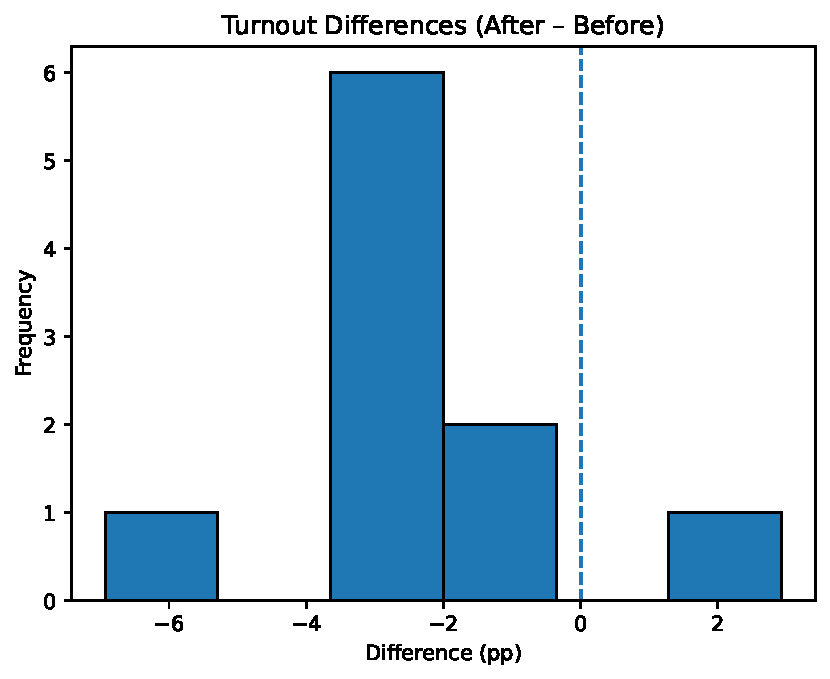
\includegraphics[width=\textwidth]{Figures/paired_diff.pdf}
\end{columns}
\end{frame}

\begin{frame}
\frametitle{Example -- Interpreting the 95\% CI}
\begin{itemize}
  \item CI for mean change: \((-3.7 \text{ pp},\;0.1 \text{ pp})\)  (pp.=percentage points).
  \item All values in this range are equally compatible with the data at the 5\% significance level
  \item \(\mathbf{You\;cannot}\) assign greater ``plausibility” to negative vs.\ positive values
  \item Conclusion: Data support a decrease, no change, or a small increase — nothing beyond this interval is consistent at 95\%
\end{itemize}
\end{frame}



% ------------------------------------------------------------------
\begin{frame}
\frametitle{Practice Problem 2 -- Paired Data, Small Sample}

\[
T \;=\;\frac{\bar d - \mu_{d,0}}{s_d/\sqrt n}\quad\sim\quad t_{\,n-1}
\]

\vspace{-0.5em}

\begin{block}{Context}
\begin{itemize}\setlength\itemsep{0.4em}
  \item \(n=9\) individuals measured \textbf{before} and \textbf{after} a training program.
  \item Goal: Test if mean improvement \(\mu_d\) differs from 0.
  \item Use a \textbf{paired \(t\)} test — small sample, assume differences $\approx$ normal.
\end{itemize}
\end{block}

\pause

\textbf{Quick practice (think–pair–share)}:\\
\(\bar d=4.1,\; s_d=5.4,\; \alpha=0.10\) (two-sided).\\
Reject \(H_0\)? → \(T = 2.27 > t^{\ast}_{\,8} = 1.86\) → \textbf{Yes}.

\end{frame}

% ------------------------------------------------------------------
% Stand-alone slide: Paired Difference – Large Sample Inference
% ------------------------------------------------------------------
\begin{frame}
\frametitle{Addendum -- Inference for Paired Differences (Large $n$)}
\small 

\textbf{Scenario:} You observe two measurements on each unit (e.g., before vs after treatment)  
and compute the difference $d_i = x_{\text{after},i} - x_{\text{before},i}$.

\vspace{0.6em}
\textbf{When $n$ is large}, we invoke the Central Limit Theorem:
\[
\bar{d} \sim N\left(\mu_d,\ \frac{\sigma_d^2}{n}\right)
\quad\text{(approximately, by CLT)}.
\]
\textbf{Use \textit{Z} procedures} if:
\begin{itemize}
  \item $n \ge 30$ (number of \textit{pairs}),
  \item Independence: pairs are randomly sampled or randomly assigned,
  \item You estimate $\sigma_d$ with sample SD ($s_d$).
\end{itemize}


\[
\textbf{CI for $\mu_d$}: \bar{d} \pm z^{\ast}_{1-\alpha/2} \cdot \frac{s_d}{\sqrt{n}}
\qquad \text{Test stat: } Z = \frac{\bar{d} - \mu_{d,0}}{s_d/\sqrt{n}}
\]

\end{frame}


% ------------------------------------------------------------
% 4.  Two‑sample inference
% ------------------------------------------------------------
\section{Two Independent Means}

\transitionslide{Comparing Two Small Samples}


%...............................................................................
% Concept slide

\begin{frame}
\frametitle{Comparing Means Using Small Samples}

\textbf{Core Question:} Do two distinct groups differ \emph{on average} in some key outcome?

\vspace{1em}
\begin{itemize}
  \item Do 12 rural precincts using new machines have shorter average wait times than 12 using the old ones?
  \item Do honors students in a pilot class (n = 14) outperform regular students (n = 15) on a civics quiz?
  \item Are turnout rates different across two small counties in a special election (n = 10 precincts each)?
\end{itemize}
\end{frame}

\begin{frame}
\frametitle{Comparing Means Using Small Samples}

\textbf{What makes this different from one-sample inference?}
\begin{itemize}
  \item Two samples = two sources of variability  
  \item Independence between groups is critical  
  \item Assumptions about spread (equal vs unequal variance) influence the method
\end{itemize}

\vspace{1em}
\pause
\textit{Our goal:} Infer whether population means \(\mu_1\) and \(\mu_2\) are different, using small samples.
\end{frame}

% ...................................................................................
\begin{frame}
\frametitle{Why Variance Matters More with Small Samples}

In large samples, we relied on the Law of Large Numbers:\\
\[
SE = \sqrt{\frac{\sigma_1^2}{n_1} + \frac{\sigma_2^2}{n_2}} \quad (\text{plug-in with } s_1, s_2)
\]

\vspace{1em}
\pause

\large
But with small samples:
\begin{itemize}
  \item Estimates \(s_1\) and \(s_2\) are noisy — not reliable stand-ins for \(\sigma_1, \sigma_2\)
  \item This extra uncertainty fattens the tails of our test statistic
  \item We need to adjust using a \textbf{t distribution} — with carefully chosen degrees of freedom
\end{itemize}
\end{frame}


% ------------------------------------------------------------------
% Stand‑alone slide: Pooled Standard Deviation (insert where needed)
% ------------------------------------------------------------------
\begin{frame}
\frametitle{When \& How to Pool Variances}

\textbf{Equal‐variance assumption}  
\(\sigma_1^2 = \sigma_2^2 = \sigma^2\) in the populations.  
A quick screen: variance (or SD) ratio $<2$ \textit{and} similar histograms.

\vspace{0.5em}
\textbf{Pooled estimate of the common SD}
\[
s_{pooled}^2 = 
s_p^2
= 
\frac{(n_1-1)s_1^{2} + (n_2-1)s_2^{2}}
     {\,n_1+n_2-2\,},
\qquad
s_p = \sqrt{s_p^2}.
\]
\[
SE_{\text{pooled}}
=
s_p\,
\sqrt{\frac{1}{n_1}+\frac{1}{n_2}},
\qquad
df = n_1+n_2-2.
\]

\begin{block}{Use pooled $t$ only when:}
\begin{itemize}
  \item Boxplots / histograms show comparable spread;\\[-0.4em]
  \item Sample sizes are not wildly unequal;\\[-0.4em]
  \item A formal test (e.g.\ Levene) does \emph{not} reject equal variances.
\end{itemize}
\end{block}

\alert{Otherwise, default to Welch’s unpooled procedure.}
\end{frame}

%...............................................................................
% Formula slide
\begin{frame}
\frametitle{Welch \textbf{t} statistic (safer default)}
\[
T \;=\;
\frac{(\bar X_1-\bar X_2) - \Delta_0}
     {\sqrt{\dfrac{S_1^2}{n_1}+\dfrac{S_2^2}{n_2}}}
\quad\sim\quad t_{df_{\text{Welch}}}
\]
\begin{block}{Welch degrees of freedom (software reports this)}
\[
df=\frac{\bigl(\tfrac{S_1^2}{n_1}+\tfrac{S_2^2}{n_2}\bigr)^2}{
      \tfrac{S_1^4}{n_1^2(n_1-1)}+\tfrac{S_2^4}{n_2^2(n_2-1)}}.
\]
\end{block}
Use pooled‐SD version only when diagnostics support equal population variances.
\end{frame}

%...............................................................................
\begin{frame}% Flowchart slide
\frametitle{Pooled vs.\ Welch decision tree}

\centering
\resizebox{\textwidth}{!}{%
\begin{tikzpicture}[
    >=Stealth,
    node distance = 1.4cm and 2.6cm,  % vertical, horizontal
    block/.style = {
        rectangle, draw, thick, rounded corners,
        align=center, minimum width=3.2cm, minimum height=1.1cm,
        inner sep=2pt
    },
    start/.style = {
        diamond, draw, thick, aspect=2, align=center,
        inner sep=2pt
    },
    edge_label/.style = {midway, sloped, font=\small, auto}
]

% ── Nodes ─────────────────────────────────────────────
\node (start) [start] {Start here};
\node (eqtest) [block, below=of start] {Variance ratio $<2$ \\ \& histograms similar?};

% Pull children inward slightly with x-shifts so the tree is tighter
\node (pooled) [block, below left=of eqtest,  xshift= .6cm] {Use pooled $t$};
\node (welch)  [block, below right=of eqtest, xshift=-.6cm] {Use Welch \\ (unpooled)};

% ── Arrows + labels ──────────────────────────────────
\draw[->, thick] (start) -- (eqtest);
\draw[->, thick] (eqtest) -- node[edge_label] {yes} (pooled);
\draw[->, thick] (eqtest) -- node[edge_label] {no}  (welch);

\end{tikzpicture}} % end resizebox
\end{frame}



% Example slide (problem statement)
\begin{frame}
\frametitle{Example — Civics Quiz Scores: Honors vs Regular}
\small
\begin{itemize}
    \item \textbf{Research context:} Instructor wants to know if an enriched honors curriculum leads to higher civics‐quiz performance than the standard curriculum  
    \item \textbf{Data:} 20‐question multiple‐choice quiz (0–100 scale), administered simultaneously to two sections in Spring term  
    \item \textbf{Goal:} Estimate and test the difference in true mean scores between honors vs.\ regular students  
    \item Honors class: \(n_1=12,\ \bar x_1=77.3,\ s_1=8.4\)  
    \item Regular class: \(n_2=15,\ \bar x_2=70.1,\ s_2=7.1\)  
    \item Hypothesis test: \(H_0: \mu_1-\mu_2 = 0\) vs.\ two‑sided \(H_a\) at \(\alpha=0.05\)
\end{itemize}
\end{frame}


% Example slide (calculation)
\begin{frame}
\frametitle{Calculations}

\[
SE=\sqrt{\frac{8.4^2}{12}+\frac{7.1^2}{15}}=3.29, 
\quad T=\frac{77.3-70.1}{3.29}=2.19
\]
\vspace{-0.3em}
\begin{align*}
df_{\text{Welch}} &=
\frac{(8.4^2/12 + 7.1^2/15)^2}{\tfrac{8.4^4}{12^2\cdot11} + \tfrac{7.1^4}{15^2\cdot14}}
\ \approx\ 20.7
\end{align*}
Two‑tailed critical value: \(t^{\ast}_{0.975,\,20}=2.086\).  
Since \(2.19>2.086\) we \textbf{reject} \(H_0\).
\vspace{0.3em}

\textbf{Conclusion}: Honors students score significantly higher ($\approx7$ pts).
\end{frame}

% Pitfalls slide
\begin{frame}
\frametitle{Common traps with two‑sample t}
\begin{itemize}
  \item \textbf{Heteroskedasticity}: ignoring unequal variances shrinks \(SE\).  
  \item \textbf{Imbalanced $n$}: smaller group sample size drives \(df\); watch power.  
  \item \textbf{Multiple testing}: comparing many sub‑groups inflates Type I error (adjust \(\alpha\) or use FDR).
\end{itemize}
\end{frame}

% ------------------------------------------------------------
% 5.  Wrap‑up summary
% ------------------------------------------------------------
\section{Summary}

% Transition slide

\transitionslide{Key Formulas and Takeaways}

%...............................................................
% Summary table
\begin{frame}
\frametitle{Cheat‑Sheet -- Small Sample Inference}
\footnotesize
\begin{table}[H]
\centering\renewcommand{\arraystretch}{3}
\resizebox{\textwidth}{!}{%
\begin{tabular}{|c|c|c|}
\hline
\textbf{Scenario} & \textbf{Confidence Interval} & \textbf{Test Statistic} ($\Delta_0$ or $\mu_0$ in numerator)\\
\hline
One mean $\mu$ &
$\displaystyle \bar x \pm t_{n-1}^{\ast}\frac{s}{\sqrt n}$ &
$\displaystyle T=\frac{\bar x-\mu_0}{s/\sqrt n}\quad(df=n-1)$\\
\hline
Paired mean $\mu_d$ &
$\displaystyle \bar d \pm t_{n-1}^{\ast}\frac{s_d}{\sqrt n}$ &
$\displaystyle T=\frac{\bar d-\mu_{d,0}}{s_d/\sqrt n}\quad(df=n-1)$\\
\hline
Two means $\mu_1-\mu_2$ (Welch) &
$\displaystyle (\bar x_1-\bar x_2)\pm t_{df}^{\ast}\sqrt{\frac{s_1^2}{n_1}+\frac{s_2^2}{n_2}}$ &
$\displaystyle T=\frac{(\bar x_1-\bar x_2)-\Delta_0}{\sqrt{\frac{s_1^2}{n_1}+\frac{s_2^2}{n_2}}}\quad(df=\text{Welch})$\\
\hline
Two means $\mu_1-\mu_2$ (Pooled) &
$\displaystyle (\bar x_1-\bar x_2)\pm t_{n_1+n_2-2}^{\ast} s_p \sqrt{\frac{1}{n_1}+\frac{1}{n_2}}$ &
$\displaystyle T=\frac{(\bar x_1-\bar x_2)-\Delta_0}{s_p\sqrt{\frac{1}{n_1}+\frac{1}{n_2}}}\quad(df=n_1+n_2-2)$\\
\hline
\end{tabular}}
\end{table}
\vspace{0.4em}
\begin{itemize}
  \item Always check independence \emph{and} approximate Normal shape.  
  \item Use Welch unless equal‑variance assumption is defensible.  
  \item Report \(df\) and \(p\)-value to two decimals.
\end{itemize}
\end{frame}


\end{document}

